% Copyright 2024 Kieran W Harvie. All rights reserved.

\section{Barycentric Coordinates}
\label{appx:bary}
\begin{center}
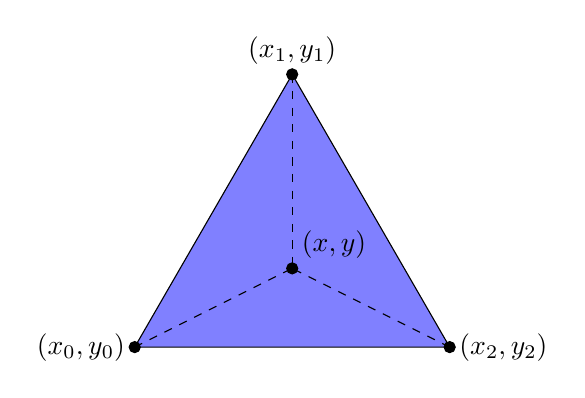
\begin{tikzpicture}[every node/.style={black}]
	\coordinate (p0) at (0,0);
	\coordinate (p1) at (4*0.5,4*0.86602540378);
	\coordinate (p2) at (4,0);
	\coordinate (p) at (2,1);

	\filldraw[fill=blue!50] (p0) -- (p1) -- (p2) -- cycle;

	\draw[dashed] (p0)--(p);
	\draw[dashed] (p1)--(p);
	\draw[dashed] (p2)--(p);

	\filldraw (p0) node[left]{$(x_0,y_0)$} circle(2pt);
	\filldraw (p1) node[above]{$(x_1,y_1)$} circle(2pt);
	\filldraw (p2) node[right]{$(x_2,y_2)$} circle(2pt);
	\filldraw (p) node[above right]{$(x,y)$} circle(2pt);
\end{tikzpicture}
\end{center}
Given three points $(x_n,y_n)$ of a triangle the barycentric coordiates for a point $(x,y)$ are numbers $\lambda_0,\lambda_1,$ and $\lambda_2$ such that:
\[(x,y) = \lambda_0(x_0,y_0)+\lambda_1(x_1,y_1)+\lambda_2(x_2,y_2)\quad \lambda_0+\lambda_1+\lambda_2=1\]
These requirements are equivalent to the following matrix equation:
\[
\begin{bmatrix}
	x_0&x_1&x_2\\
	y_0&y_1&y_2\\
	1&1&1\\
\end{bmatrix}
\begin{bmatrix}
	\lambda_0\\\lambda_1\\\lambda_2\\
\end{bmatrix}
=
\begin{bmatrix}
	x\\y\\1\\
\end{bmatrix}
\]
To analyse this equation start by considering the following identity: 
\[
\begin{vmatrix}
	a_0&a_1&a_2\\
	b_0&b_1&b_2\\
	1&1&1\\
\end{vmatrix}
=
\begin{vmatrix}
	a_0&a_1-a_0&a_2-a_0\\
	b_0&b_1-b_0&b_2-b_0\\
	1&0&0\\
\end{vmatrix}
=
\begin{vmatrix}
	a_1-a_0&a_2-a_0\\
	b_1-b_0&b_2-b_0\\
\end{vmatrix}
\]
This means that the normal requirement for a solution,
that the determinate of the matrix be nonzero,
is equivalent to:
\[
	0\neq
\begin{vmatrix}
	x_0&x_1&x_2\\
	y_0&y_1&y_2\\
	1&1&1\\
\end{vmatrix}
\Leftrightarrow
0\neq
\begin{vmatrix}
	x_1-x_0&x_2-x_0\\
	y_1-y_0&y_2-y_0\\
\end{vmatrix}
\]
It also lets us simplify the solutions for $\lambda_n$ obtained through Cramer's rule:
\[
	\lambda_0 = 
\frac
{\begin{vmatrix}
	x&x_1&x_2\\
	y&y_1&y_2\\
	1&1&1\\
\end{vmatrix}}
{\begin{vmatrix}
	x_0&x_1&x_2\\
	y_0&y_1&y_2\\
	1&1&1\\
\end{vmatrix}}
=
\frac
{\begin{vmatrix}
	x_1-x&x_2-x\\
	y_1-y&y_2-y\\
\end{vmatrix}}
{\begin{vmatrix}
	x_1-x_0&x_2-x_0\\
	y_1-y_0&y_2-y_0\\
\end{vmatrix}}
\]
These results can be interpreted geometrically,
firstly is that a solution exist if and only if the set $\{(x_1-x_0,y_1-y_0),(x_2-x_0,y_2-y_0)\}$ is linearly independent.
Note that this isn't the same as $\{(x_0,y_0),(x_1,y_1),(x_2,y_2)\}$ being linearly independent,
as two points can be on the same line through the origin so long as the third isn't:
\begin{center}
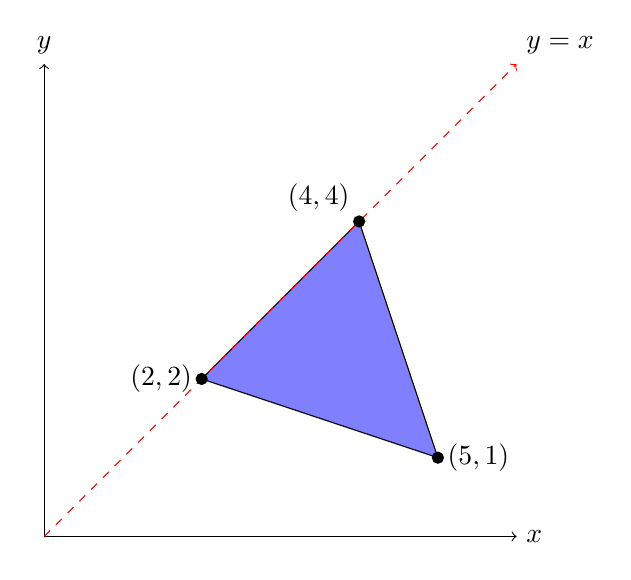
\begin{tikzpicture}[every node/.style={black}]
	\draw[<->] (0,6) node[above]{$y$} -- (0,0) -- (6,0) node[right] {$x$};

	\coordinate (p0) at (2,2);
	\coordinate (p1) at (4,4);
	\coordinate (p2) at (5,1);
	\coordinate (O) at (0,0);

	\filldraw[fill=blue!50] (p0) -- (p1) -- (p2) -- cycle;

	\draw[->, dashed,red] (0,0) -- (6,6) node[above right]{$y=x$};

	\filldraw (p0) node[left]{$(2,2)$} circle(2pt);
	\filldraw (p1) node[above left]{$(4,4)$} circle(2pt);
	\filldraw (p2) node[right]{$(5,1)$} circle(2pt);
\end{tikzpicture}

An example valid triangle with two points lying on the same $y=x$ line.
\end{center}
Secondly is that $\begin{vmatrix}x_1-x&x_2-x\\y_1-y&y_2-y\\\end{vmatrix}$ can be interpreted as the (signed) area of the parallelogram defined by the points $(x_1,y_1)$ and $(x_2,y_2)$ with origin $(x,y)$\footnote{This follows from $\begin{vmatrix}x_1&x_2\\y_1&y_2\\\end{vmatrix}$ being the singed area of the parallelogram of the points $(x_1,y_1)$ and $(x_2,y_2)$ through the origin}.
This means that, 
when $(x,y)$ is contained within the triangle,
$\lambda_0$ can be interpreted as the fraction of the of area the triangle $\{(x,y),(x_1,y_1),(x_2,y_2)\}$ to the area of the larger triangle.
This is why barycentric coordinate are some times called area coordinates. 

\begin{center}
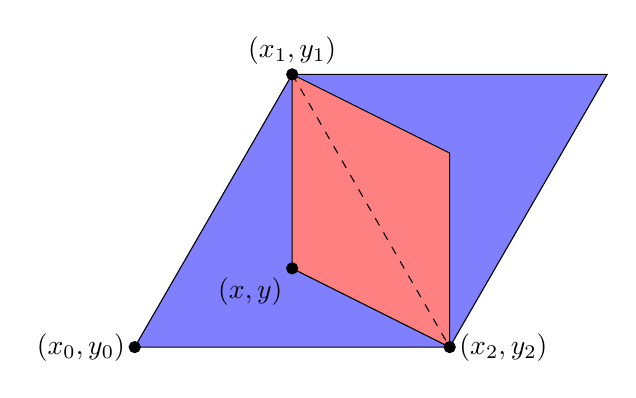
\begin{tikzpicture}[every node/.style={black}]
	\coordinate (p0) at (0,0);
	\coordinate (p1) at (4*0.5,4*0.86602540378);
	\coordinate (p2) at (4,0);
	\coordinate (p3) at (6,4*0.86602540378);
	\coordinate (p) at (2,1);
	\coordinate (r) at (6-2,4*0.86602540378-1);

	\filldraw[fill=blue!50] (p0) -- (p1) -- (p3) -- (p2) --cycle;
	\filldraw[fill=red!50] (p) -- (p1) -- (r) -- (p2) --cycle;

	\filldraw (p0) node[left]{$(x_0,y_0)$} circle(2pt);
	\filldraw (p1) node[above]{$(x_1,y_1)$} circle(2pt);
	\filldraw (p2) node[right]{$(x_2,y_2)$} circle(2pt);
	\filldraw (p) node[below left]{$(x,y)$} circle(2pt);

	\draw[dashed] (p1)--(p2);
\end{tikzpicture}

Visualization of the area properties of barycentric coordinate. 
Observe the shared diagonal that lets us evenly covert the parallelograms to triangles and that the two areas have the same sign.
\end{center}
Finally these arguments can be generalized to other dimensions by making natural modification to the original matrix equation,
three dimensions would give:
\[
\begin{bmatrix}
	x_0&x_1&x_2&x_3\\
	y_0&y_1&y_2&y_3\\
	z_0&z_1&z_2&z_3\\
	1&1&1&1\\
\end{bmatrix}
\begin{bmatrix}
	\lambda_0\\\lambda_1\\\lambda_2\\\lambda_3\\
\end{bmatrix}
=
\begin{bmatrix}
	x\\y\\z\\1\\
\end{bmatrix}
\]
And one would give:
\[
\begin{bmatrix}
	x_0&x_1\\
	1&1\\
\end{bmatrix}
\begin{bmatrix}
	\lambda_0\\\lambda_1\\
\end{bmatrix}
=
\begin{bmatrix}
	x\\1\\
\end{bmatrix}
\]

